\documentclass{beamer}
\usepackage{listings}
\usepackage{enumerate}
\usepackage{amsmath}
\usepackage{amssymb}
\usepackage{tikz}
\usepackage{graphicx}
\usetheme{Boadilla}
\title[Remedying the eval that men do]
{Remedying the eval that men do}
\date{November 28, 2012}

\author[Jensen et al.]{Simon Holm Jensen, Peter A. Jonsson, Anders M{\o}ller}
\begin{document}

\AtBeginSection[]
{
    \begin{frame}{Table of Contents}
        \tableofcontents[currentsection]
    \end{frame}
}

\begin{frame}
\nocite{Remedying}
\nocite{Eval}
\titlepage
\begin{center}
Presented by Ismail Badawi
\end{center}
\end{frame}

\begin{frame}{Table of Contents}
\tableofcontents
\end{frame}

\begin{frame}{What are we talking about?}
\begin{itemize}
\item Remedying the eval that men do, ISSTA 2012
\item {\tt eval} is ``wild''; JavaScript static analyzers tend not to
handle it, resulting in inprecise data
\item Recent study shows that in practice, most real-world uses of
{\tt eval} are actually not too hard to reason about
\item Premise: want to make JavaScript more amenable to static analysis
by transforming code to eliminate calls to {\tt eval}
\item Paper presents \emph{Unevalizer}, a tool that eliminates calls
to {\tt eval} as a source-to-source transformation
\end{itemize}
\end{frame}

\section{{\tt eval}, and {\tt eval} in JavaScript}
\begin{frame}{{\tt eval}}
\begin{itemize}
\item Many programming environments provide an {\tt eval}
function, which evaluates code as a string
\item For interpreted languages, the interpreter can just call itself
\item Compiled languages can also have {\tt eval}
\end{itemize}
\end{frame}

\begin{frame}{{\tt eval} is evil}
While {\tt eval} is very powerful, it's also very dangerous.
\begin{itemize}
\item Security concerns from executing untrusted user input
\item Unpredictable side-effects
\item Confuses static analysis; some dataflow analysis can help to
determine what code is executed but not in general
\end{itemize}
\end{frame}

\begin{frame}{{\tt eval} is widely used}
\begin{itemize}
\item The eval that men do, Richards et al., ECOOP 2011
\item "We have recorded the behaviour of 337 MB of strings given as
arguments to 550,358 calls to the {\tt eval} function exercised in over
10,000 web sites."
\item Classified uses of {\tt eval} based on the arguments passed to it
\item Concluded that in many cases (as many as 83\%), the call could be
rewritten to use less dynamic language features
\end{itemize}
\end{frame}

\begin{frame}[fragile]{Example}
\begin{verbatim}
function _var_exists(name) {
    // return whether name exists in global scope
    try {
        eval('var foo = ' + name + ';');
    } catch (e) {
        return false;
    }
    return true;
}
\end{verbatim}
\pause
\vspace{5mm}
Equivalent to: {\tt name in window}.

Except the first way won't work if {\tt name} is {\tt name} or {\tt foo}. 
It's also much slower.
\end{frame}

\begin{frame}{Example (2)}

{\tt eval('window.' + key + ' = \{\};'); }

\pause
\vspace{5mm}
Equivalent to: {\tt window[key] = \{\};}

Except it won't work if {\tt key} is not a valid identifier. Again it's
also much slower.

\end{frame}

\begin{frame}{{\tt eval} in JavaScript}

Two big uses of {\tt eval} in JavaScript are
\begin{itemize}
\item Dynamic code loading. ``Importing'' code can be done by
fetching it from a server and evaluating it.
\begin{itemize}
\item Useful since code that the user doesn't need isn't downloaded
\item This is fine; the goal is to make the JavaScript
amenable to static analysis, not to eliminate {\tt eval} just because. 
We can assume we have access to all the code.
\end{itemize}
\item JSON parsing
\begin{itemize}
\item Authors published a prior paper on using string analysis to try
and determine which strings contained JSON data.
\end{itemize}
\end{itemize}
\end{frame}

\begin{frame}{Richards et al. revisited}
Using tools made available by Richards et al., authors examined Alexa top
10,000 websites and found that
\begin{itemize}
\item 6,465 of them use {\tt eval}.
\item 3,378 use it for purposes other than the previous two cases.
\item 2,589 call it with non-constant arguments.
\end{itemize}
Their conclusion: "Although {\tt eval} is pervasive, we can expect that
relatively few web sites (around 25\%) use {\tt eval} in ways that are
truly challenging to reason about with static analysis."
\end{frame}

\begin{frame}{Distribution of {\tt eval} call sites}
Looked at 17,665 static call sites, and found
\begin{itemize}
\item 3,339 used for loading library code
\item 2,202 used for parsing JSON data
\item 6,228 have constant string arguments
\item 3,624 are performing a single operation, e.g. property read/write,
{\tt typeof} check, function call
\item This suggests that a technique that handles constants, JSON, and
single operations will cover the majority of the call sites.
\end{itemize}
\end{frame}

\section{Unevalizer}

\begin{frame}{Basic approach}
Obviously, to reliably eliminate {\tt eval}, we have to precisely
approximate the code string that is passed to it. \vspace{5mm}

The basic idea is to use dataflow analysis to keep track of what data
flows into what variables and functions; if we detect that data is flowing
into a function call $F(E)$, where the expression $F$ has {\tt eval} as
one of its possible values, then a transformation component $T$ is
triggered to eliminate the call. \vspace{5mm}

$T$ either succeeds and returns a string containing equivalent
{\tt eval}-free code for $F(E)$, or fails and returns a sentinel value
in which we case we abort. \vspace{5mm}

When the analysis' least fixed point is reached, all reachable
calls to {\tt eval} have been eliminated.
\end{frame}

\begin{frame}{The transformation component}
The analysis provides the transformation component with an 8-tuple
$(E, V, D_G, D_L, D_M, r, p, n)$, where
\begin{itemize}
\item $E$ is the argument expression (in $F(E)$ from last slide)
\item $V$ is the abstract value for $E$, a sound approximation for the
code string to be evaluated
\item $D_G$ and $D_L$ are sets of names in global and local scope,
respectively
\item $D_M$ is the set of names of built-in properties that may have been
modified by the application code
\item $r$ is a boolean flag indicating whether the return value of
{\tt eval} is used or not
\item $p$ is a boolean flag indicating whether {\tt eval} is called
directly or through an alias
\item $n$ is the {\tt eval} nesting depth
\end{itemize}
\end{frame}

\begin{frame}[fragile]{Constant arguments}
It turns out {\tt eval} is often called with constant arguments. But
handling this is not as simple as it seems, i.e. you can't just 
``drop the quotes'' and replace {\tt eval("S")} by {\tt S} in general.
\vspace{5mm}

For instance, {\tt eval} returns the value of the last evaluated expression,
but can contain arbitrary statements: \vspace{3mm}

{\tt x = a() * eval('b(); c();') * d();}
\vspace{3mm}

To generate syntactically correct code and still maintain the order of
evaluation, need something like

\begin{verbatim}
var t1 = a();
b();
var t2 = c();
x = t1 * t2 * d();
\end{verbatim}
\end{frame}
\begin{frame}[fragile]{Other problems with dropping the quotes}
\begin{verbatim}
var x = 2;                var x = 2;
function f() {            function f() {
  var y = x;                var y = x;
  eval('var x;');           var x;
  return y;                 return y;
}                         }
\end{verbatim}
The function on the left returns 2, but the one on the right returns
{\tt undefined}, because variable declarations are hoisted up by the parser
to the top of the lexical scope.
\end{frame}

\begin{frame}{An extra quirk in JavaScript}
In JavaScript, {\tt eval} has a little extra quirk. \vspace{5mm}

{\tt eval('var x = 5;'); // declares x in current scope} \vspace{5mm}

{\tt var myeval = eval;} \\
{\tt myeval('var x = 5;') // declares x in *global* scope} \vspace{5mm}

{\tt eval} has different semantics depending on whether it's called
directly or through an alias! \vspace{5mm}

This is what the $p$ argument to the transformation component represents.
The latter case should be translated to {\tt g.x = 5; }, where {\tt g} is
a reference to the global object.
\end{frame}

\begin{frame}{Aside: {\tt this} in JavaScript}
The keyword {\tt this} in JavaScript can be confusing, because what it
refers to depends on how the current function was called. Consider: \vspace{2mm}

{\tt function getThis() \{ return this; \}}
\vspace{2mm}

\begin{enumerate}
\item {\tt getThis();} \\
{\tt // returns the global object (window)}
\item {\tt (\{getThis: getThis\}).getThis();} \\
{\tt // returns the receiver}
\item {\tt new getThis();} \\
{\tt // returns a new object}
\item {\tt getThis.apply('x');} or {\tt getThis.call('x')} \\
{\tt // returns the first argument }
\end{enumerate}
\end{frame}

\begin{frame}{Getting at the global object}
The first case helps lets us get a reference to the global object: \\ 
{\tt var g = (function() \{ return this; \})()}  \vspace{5mm}

Then we can transform {\tt myeval('x = 5;')} to {\tt g.x = 5}. \vspace{5mm}

This works for property writes, but not reads; accessing a nonexistent
variable throws a {\tt ReferenceError}, but reading a nonexistent
property just yields {\tt undefined}. Then a sound replacement for
{\tt myeval('x')} is not {\tt g.x} but \vspace{5mm}

{\tt ('x' in g ? g.x : throw new ReferenceError())}
\end{frame}

\begin{frame}{Other edge cases}
\begin{itemize}
\item It's possible the code string passed to {\tt eval} is not valid
JavaScript.  In that case, we can replace the call to {\tt eval} with
{\tt throw new SyntaxError()}.
\item Even if we know the entire string we can't necessarily know the
return value, e.g. {\tt eval('2; if (b) 3;')}. Unevalizer doesn't handle
this. If the return value is needed (the $r$ flag) and it's ambiguous what
it is, it aborts.
\end{itemize}
\end{frame}

\begin{frame}[fragile]{Handling non constant strings: constant propagation}
Beyond constant strings, obviously the first thing to try is constant
propagation. 

\begin{verbatim}
var json = '<large constant string>';
...
eval('area=' + json);
\end{verbatim}
\end{frame}

\begin{frame}{Handling non constant strings: JSON}
A common pattern is {\tt eval('(' + v + ')')} where {\tt v} contains JSON
data; this forces $v$ to be evaluated as an expression. \vspace{5mm}

Most modern browsers provide the {\tt JSON.parse} function as a safe
alternative to {\tt eval} for parsing JSON. We can translate the above
to {\tt JSON.parse(v)} if we can determine {\tt v} contains JSON.
\vspace{5mm}

This was the subject of prior work by the authors. Can identify JSON in
constant strings, and from calls to {\tt JSON.stringify}, and in some
cases rely on user annotations (for e.g. Ajax calls), and propagate that
information along the dataflow analysis.
\end{frame}

\begin{frame}{Handling non constant strings: tracking valid identifiers}
Property reads ({\tt eval('foo.' + x)}) can be
transformed into {\tt foo[x]}, but only if {\tt x} contains a valid
identifier. Can treat this similarly as the previous case, by tracking
which strings contain valid identifiers and propagating that information.

\vspace{5mm}

This also works for things like {\tt eval('foo\_' + x)} or otherwise
dynamically constructing identifier names; we can track which strings
contain partial identifiers (same rules as for identifiers but can e.g.
start with a number).
\end{frame}

\begin{frame}[fragile]{Handling non constant strings: specialization}
Consider the following ({\tt /x/} denotes a regex literal):
\vspace{5mm}
\begin{verbatim}
has_cookie = function(name) {
    var ca = document.cookie.split(';');
    for (var i = 0; i < ca.length; i++) {
        if (eval('ca[i].match(/\\b' + name + '=/)'))
            return true;
    }
    return false;
}
\end{verbatim}
where {\tt has\_cookie} is later called with constant cookie names,
e.g. {\tt has\_cookie('\_jsuid')}, {\tt has\_cookie('notrack')} etc. We
can gather up all the possible values for {\tt name} and have the
the conditional dispatch on them.
\end{frame}
             
\section{Evaluation}

\begin{frame}{Implementation}
\begin{itemize}
\item The transformation component was implemented against TAJS, an existing
dataflow analyzer for JavaScript.
\item The transformation component works by taking the abstract value $V$,
adding placeholders to turn it into a valid JavaScript program, parsing it,
and applying the transformation on the resulting AST, then pretty-printing
it and returning that.
\end{itemize}
\end{frame}

\begin{frame}{Benchmarks}
\begin{itemize}
\item Selected benchmarks from the Alexa top 500 list
\item Focused on the challenging cases; excluded web sites that e.g.
only use {\tt eval} to load libraries, or only parse JSON as that has
already been covered in prior work
\item Left with 19 web sites
\end{itemize}
\end{frame}

\begin{frame}{Slicing}
The 19 benchmarks selected are quite large, and TAJS, the dataflow analysis
framework used, is not able to analyze them. \vspace{5mm}

To evaluate the Unevalizer, 25 interesting program slices (calls to
{\tt eval} and the relevant dataflow) were manually extracted from the
benchmarks. \vspace{5mm} 

Also added three interesting Chrome Experiments that use {\tt eval} in
interesting ways, resulting in 28 benchmarks.
\end{frame}  

\begin{frame}{Research questions}
\begin{enumerate}
\item Is the Unevalizer able to transform common usage patterns of
{\tt eval} calls?
\item To what extent are the individual techniques presented (constant
propagation, tracking valid identifiers, specialization) useful in practice?
\item For call sites where the Unevalizer fails to find a valid
transformation, can we suggest improvements that are likely to handle
more cases?
\end{enumerate}
\end{frame}

\begin{frame}{Results}
\begin{columns}[l]
\column{1.5in}
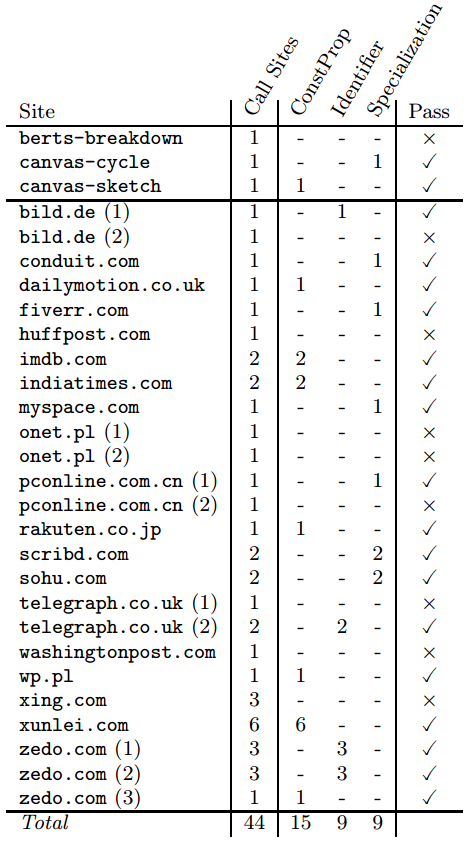
\includegraphics[scale=0.25]{results.png}
\column{3in}
\begin{itemize}
\item Pass: whether Unevalizer was able to eliminate all calls to
{\tt eval} in this benchmark (19/28, or 33/44 call sites)
\item ConstProp/Identifier/Specialization: how many call sites are handled
by each technique
\end{itemize}
\end{columns}
\end{frame}

\begin{frame}[fragile]{Example successful transformation}
\begin{verbatim}
function _SoAD_exec(o) {
  if (eval("typeof(" + o.t + "_main)") == "function")
    eval(o.t + "_main(o)");
}
function _SoAD_exec(o) {
  if (typeof(
        (o.t + "_main") in global ?
            global[o.t + "_main"] :
            throw new ReferenceError())
      == "function")
     ((o.t + "_main") in global ?
          global[o.t + "_main"] :
            throw new ReferenceError())(o);
}
\end{verbatim}
Safe because the dataflow analysis determines {\tt o.t} always contains
a valid identifier.
\end{frame}

\begin{frame}[fragile]{Cause for failure: insufficient precision}
\begin{verbatim}
for (var libName in $iTXT.js.loader) {
  eval(libName + '_Load()');
}
\end{verbatim}
\vspace{5mm}
{\tt \$iTXT.js.loader} keys refer to modules; some of them contain dots, 
so aren't valid identifiers, so the call site can't be transformed.

\vspace{5mm}
Could apply loop unrolling, enabling many of the calls to be transformed.
\end{frame}

\begin{frame}[fragile]{Cause for failure: string concatenation}
The analysis has special treatment of string concatenations as arguments
to functions. In this example:

\begin{verbatim}
function showIvyViaJs(locationId) {
  ...
  var _fconv = "ivymap[\'" + locationId + "\'";
  try {
    _f = eval(_fconv);
    ...
  } catch (e) {}
}
\end{verbatim}
\vspace{5mm}
The analysis doesn't determine that {\tt \_fconv} could be specialized on.
Could improve constant propagation to propagate entire expressions.
\end{frame}

\begin{frame}{Conclusion}
"The {\tt eval} function is in practice not as evil as some men claim."
\vspace{5mm}
Unevalizer succeeds in eliminating typical uses of {\tt eval}, but
possible improvements are many; future work includes better handling of
{\tt eval} in loops, extending constant propagation, and generally improving
the precision of the string analysis.
\end{frame}

\begin{frame}{References}
\bibliographystyle{plain}
{\footnotesize
\bibliography{bib}}
\end{frame}

\end{document}
